\documentclass[UTF8]{ctexart}
\usepackage{bm}
\usepackage{amssymb}
\usepackage{mathtools}
\usepackage{amsmath}
\usepackage{float}
\usepackage{rotating}
\usepackage{booktabs}
\usepackage{pdfpages}
\usepackage{pgf,tikz}
\usepackage{mathrsfs}
\usetikzlibrary{arrows}
\title{\heiti 最优化第八次作业}
\author{\kaishu 张晋15091060}
\begin{document}
\maketitle
\begin{enumerate}
\item[3.7]
\begin{enumerate}
\item 用$x_{ij}$代表在城市$j$设置工厂$i$,则有:
\begin{alignat}{2}
min \quad & \sum_i^n\sum_k^n\sum_j^n\sum_l^n t_{ik}d_{jl}x_{ij}x_{kl}  \nonumber\\
\mbox{s.t.}\quad    &\sum_i^n x_{ij}=1 \qquad(j=1,\cdots,n) 
\nonumber\\
&\sum_j^n x_{ij}=1 \qquad(i=1,\cdots,n) 
\nonumber\\
&x_{ij}\in {0,1}\qquad (i,j=1,\cdots,n) 
\end{alignat}

\item 由于极小化的目标函数中交叉项系数都为正,故可用$y_{ijkl}$来代替$x_{ij}x_{kl}$,其中$y_{ijkl}$满足
\[y_{ijkl} \geq x_{ij}+x_{kl}-1,\quad y_{ijkl} \geq 0\]

故原规划转化为线性规划如下:
\begin{alignat}{2}
min \quad & \sum_i^n\sum_k^n\sum_j^n\sum_l^n t_{ik}d_{jl}y_{ijkl}  \nonumber\\
\mbox{s.t.}\quad    &\sum_i^n x_{ij}=1 \qquad(j=1,\cdots,n) 
\nonumber\\
&\sum_j^n x_{ij}=1 \qquad(i=1,\cdots,n) 
\nonumber\\
&x_{ij}\in {0,1}\qquad (i,j=1,\cdots,n)\nonumber \\
&y_{ijkl} \geq x_{ij},\quad y_{ijkl} \geq 0\qquad(i,j,k,l=1,\cdots,n) 
\end{alignat}
\end{enumerate}

\item[3.8]$P_0$的最优单纯形表为:

\begin{table}[H]
\centering
	\begin{tabular}{ccccc}
	\toprule
	{}&$x_1$&$x_2$&$x_3$&$\bm{B}^{-1}\bm{b}$\\
	\midrule
     {}    & 1    & 1/2     & -1/4    &5/4 \\
       $\bm{r}^T$     & 0     & 3/2     & 1/4     & -5/4    \\
	\bottomrule
	\end{tabular}
\end{table}

给$P_0$添加约束$x_1\geq2$得:

\begin{table}[H]
\centering
	\begin{tabular}{cccccc}
	\toprule
     	{}&$x_1$&$x_2$&$x_3$&$x_4$&$\bm{B}^{-1}\bm{b}$\\
	\midrule
     {}   & \boxed{1}    & 1/2     & -1/4   &0 &5/4 \\
     {}    & 1    & 0    & 0    &-1 &2 \\
     $\bm{r}^T$     & 0     & 3/2     & 1/4   &0  & -5/4    \\
	\bottomrule
	\end{tabular}
\end{table}

\begin{table}[H]
\centering
	\begin{tabular}{cccccc}
	\toprule
     	{}&$x_1$&$x_2$&$x_3$&$x_4$&$\bm{B}^{-1}\bm{b}$\\
	\midrule
	  {}    & 1    & 1/2     & -1/4   &0 &5/4 \\
     {}    & 0    & 1/2     & \boxed{-1/4}   &1 &-3/4 \\
     $\bm{r}^T$     & 0     & 3/2     & 1/4   &0  & -5/4    \\
	\bottomrule
	\end{tabular}
\end{table}

\begin{table}[H]
\centering
	\begin{tabular}{cccccc}
	\toprule
     	{}&$x_1$&$x_2$&$x_3$&$x_4$&$\bm{B}^{-1}\bm{b}$\\
	\midrule
	  {}    & 1    & 0     & 0   &-1 &2 \\
     {}    & 0    & -2     & 1   &-4 &3\\
     $\bm{r}^T$     & 0     & 2    & 0   &1  & -2 \\
	\bottomrule
	\end{tabular}
\end{table}

得最优解$\bm{x}=(2,0,3,0)^T$,最优值为2.

\item[3.9]
由图解法可得:
问题(i)的解为$(1.5,3)$,问题(ii)的解为$(2,2.5)$,问题(iii)的解为$(2,2)$.

分支定界法采用深度优先搜索,详细内容见枚举树.

\begin{figure}[H]
\small
\centering
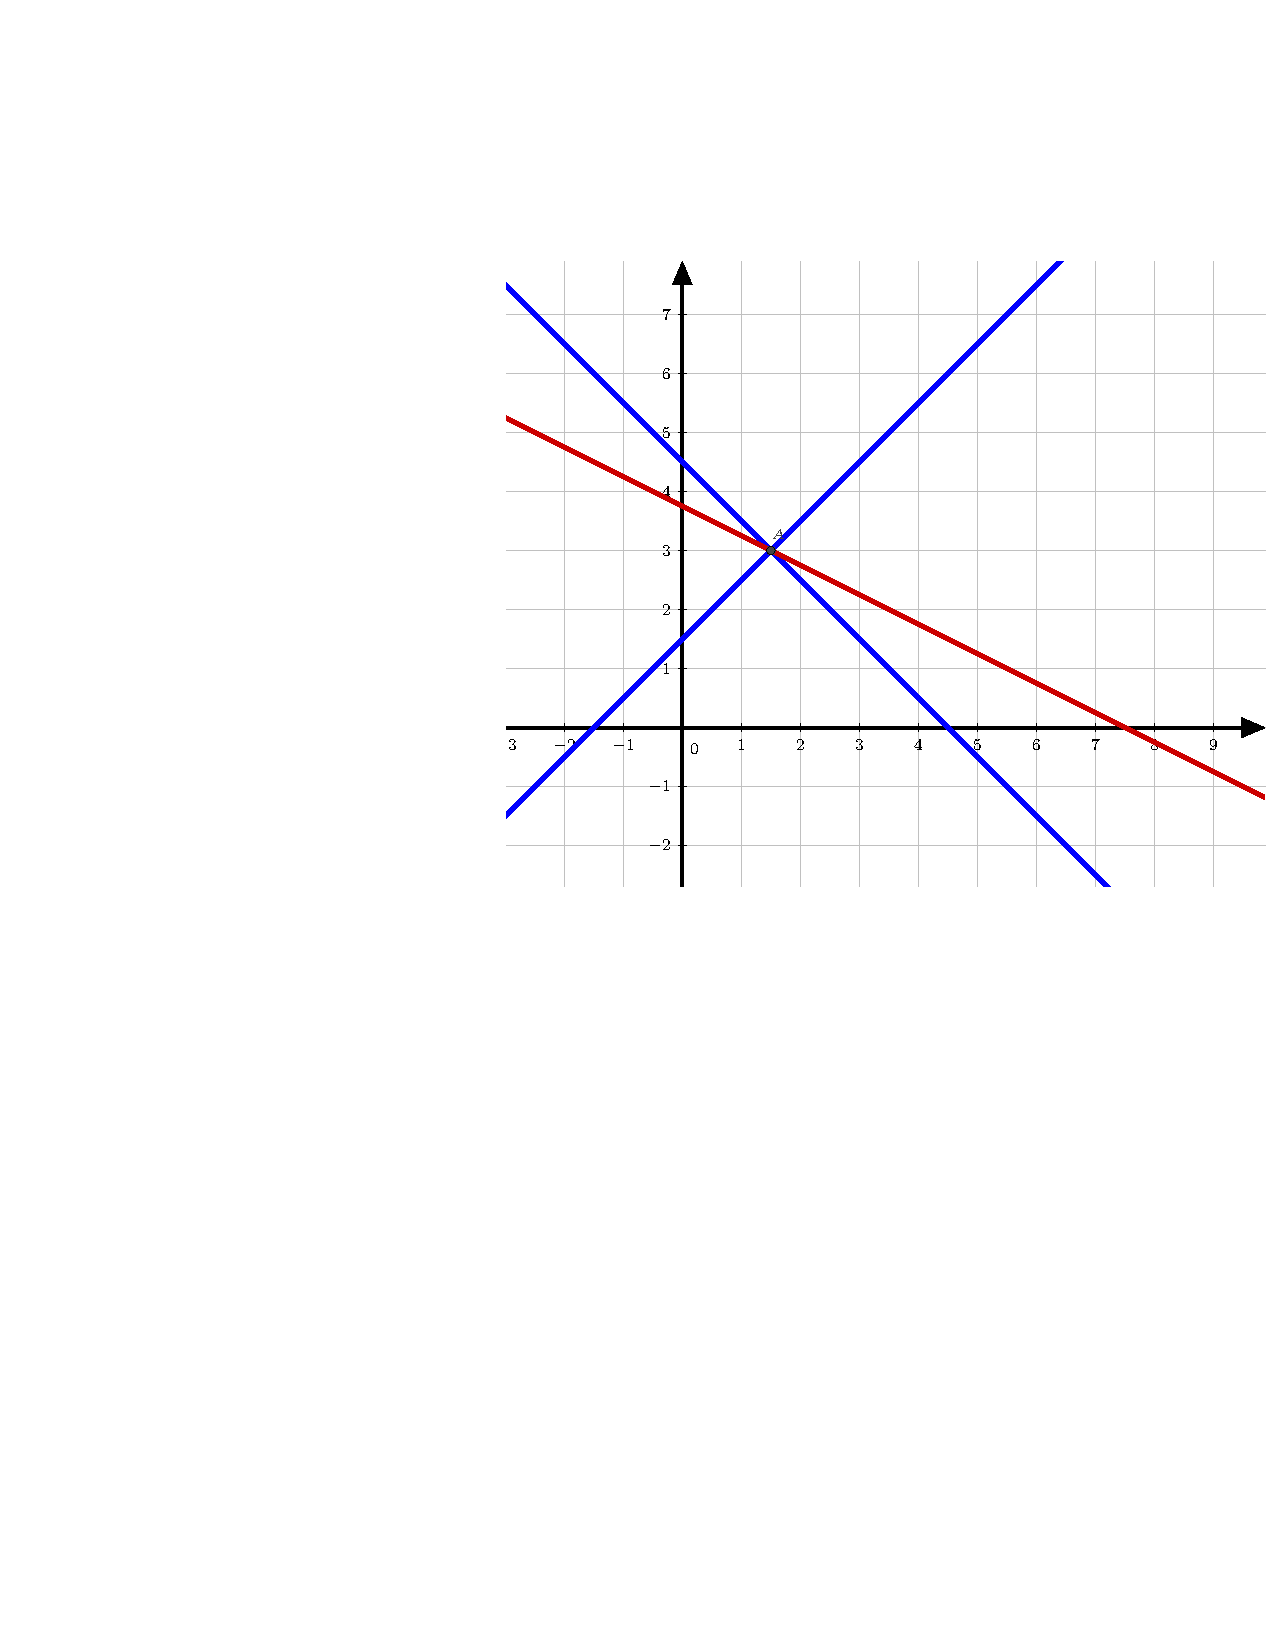
\includegraphics[width=9cm]{1.pdf}
\caption{无整数限制}
\end{figure}

\begin{figure}[H]
\small
\centering
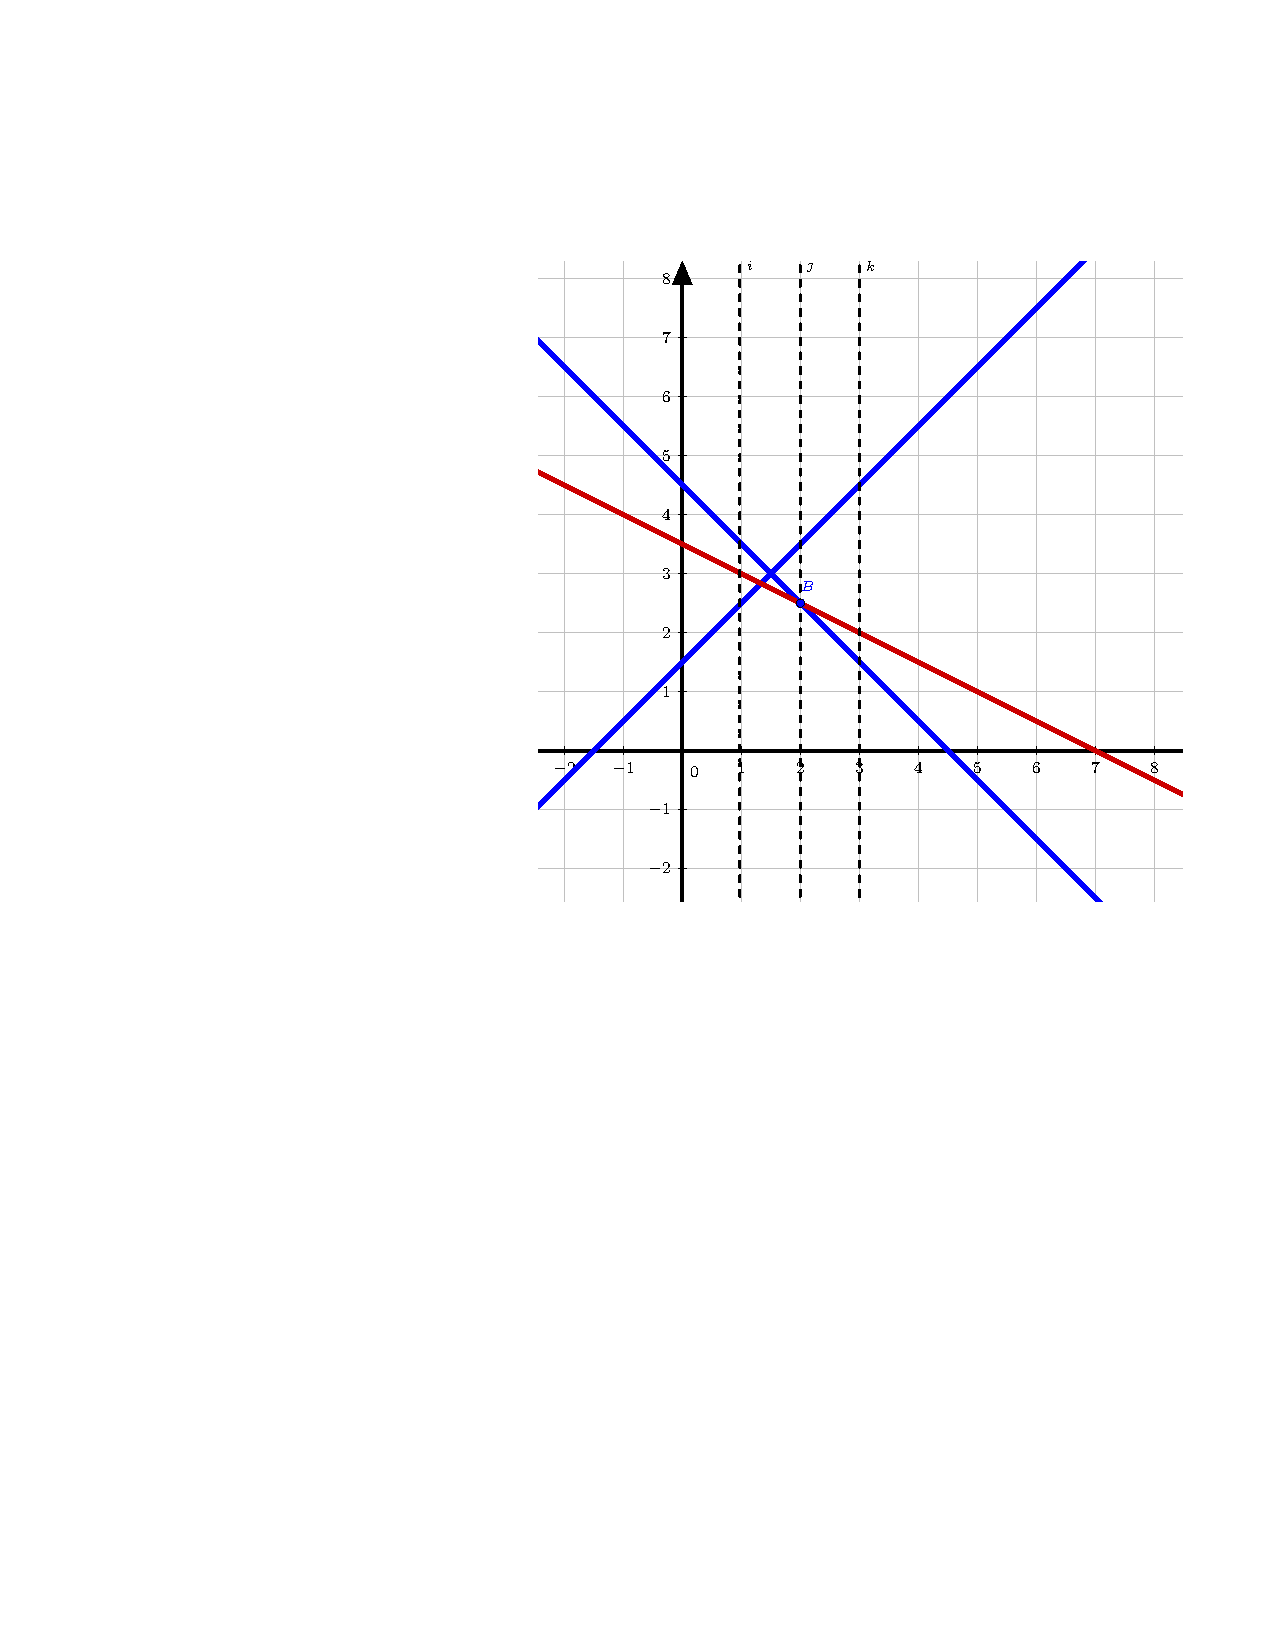
\includegraphics[width=9cm]{2.pdf}
\caption{$x_1$为整数}
\end{figure}

\begin{figure}[H]
\small
\centering
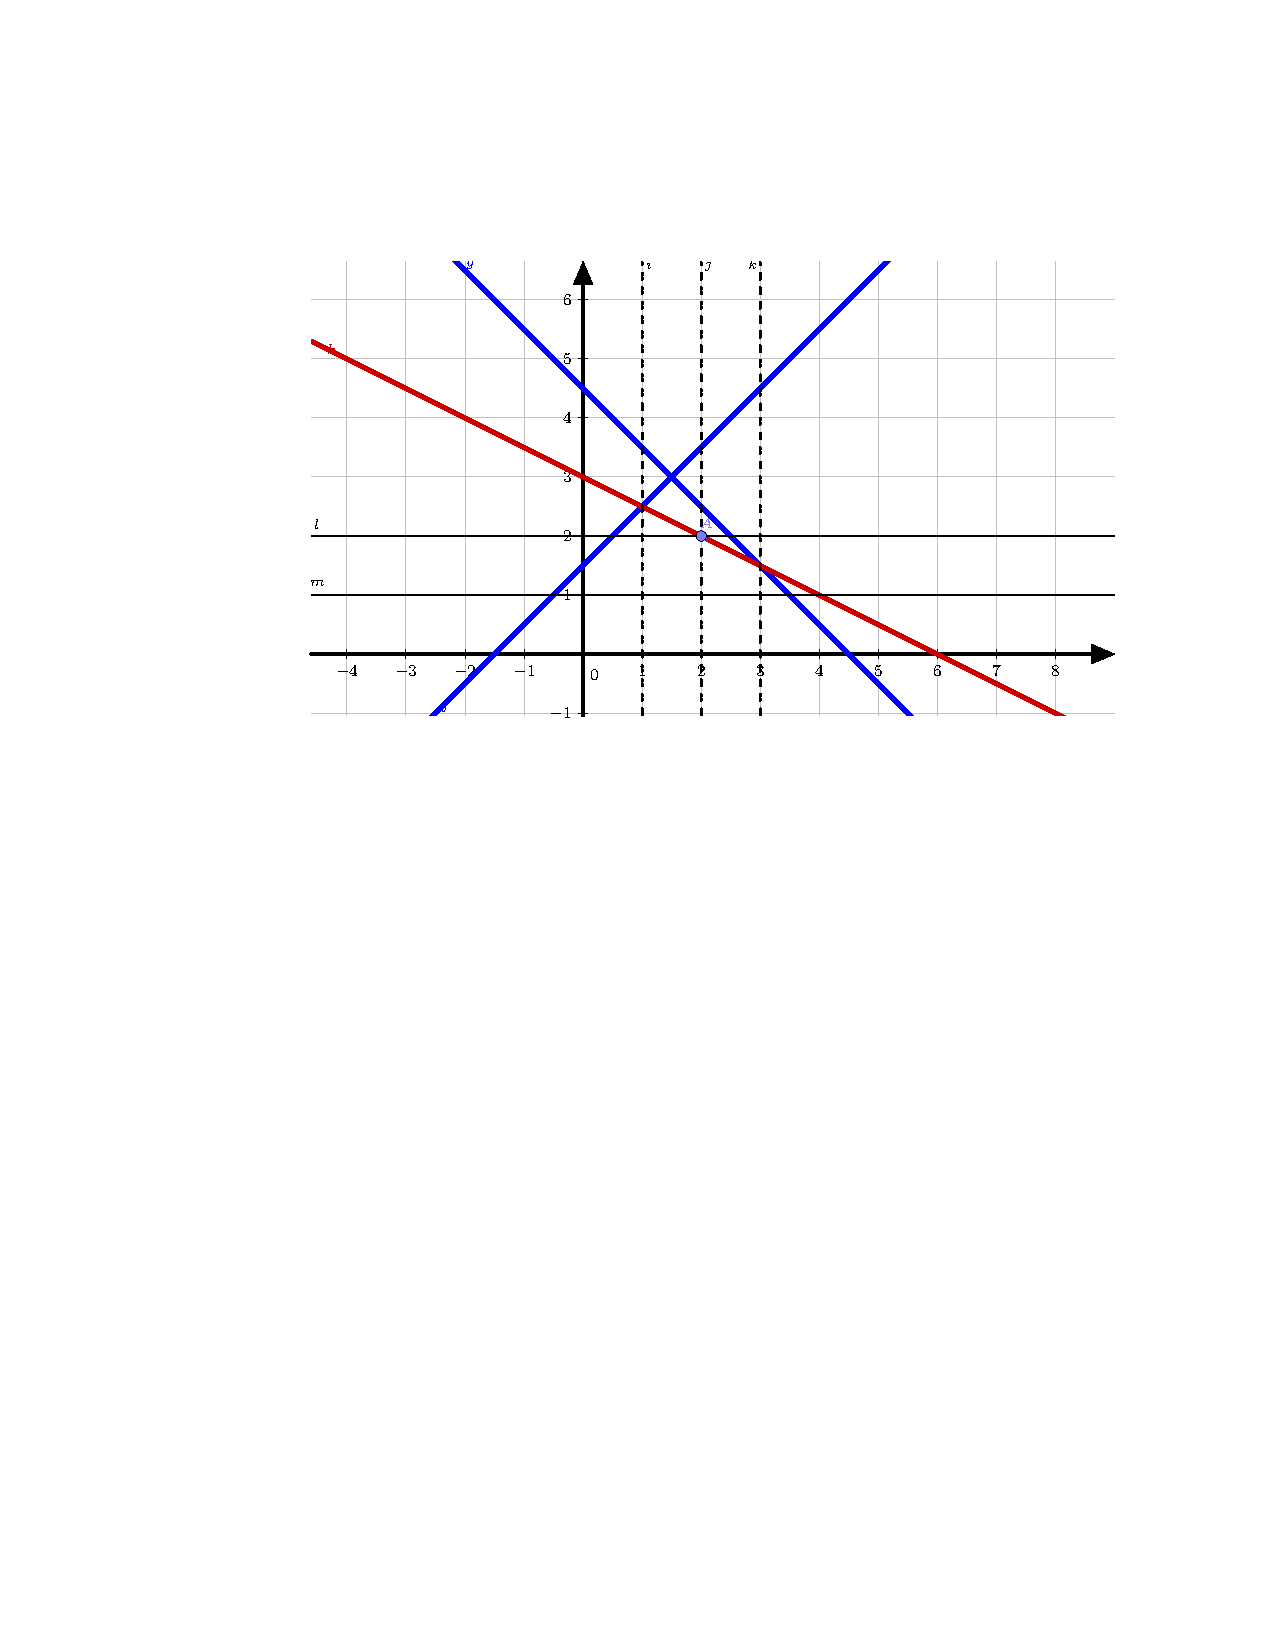
\includegraphics[width=12cm]{3.pdf}
\caption{$x_1,x_2$为整数}
\end{figure}

\begin{figure}[H]
\small
\centering
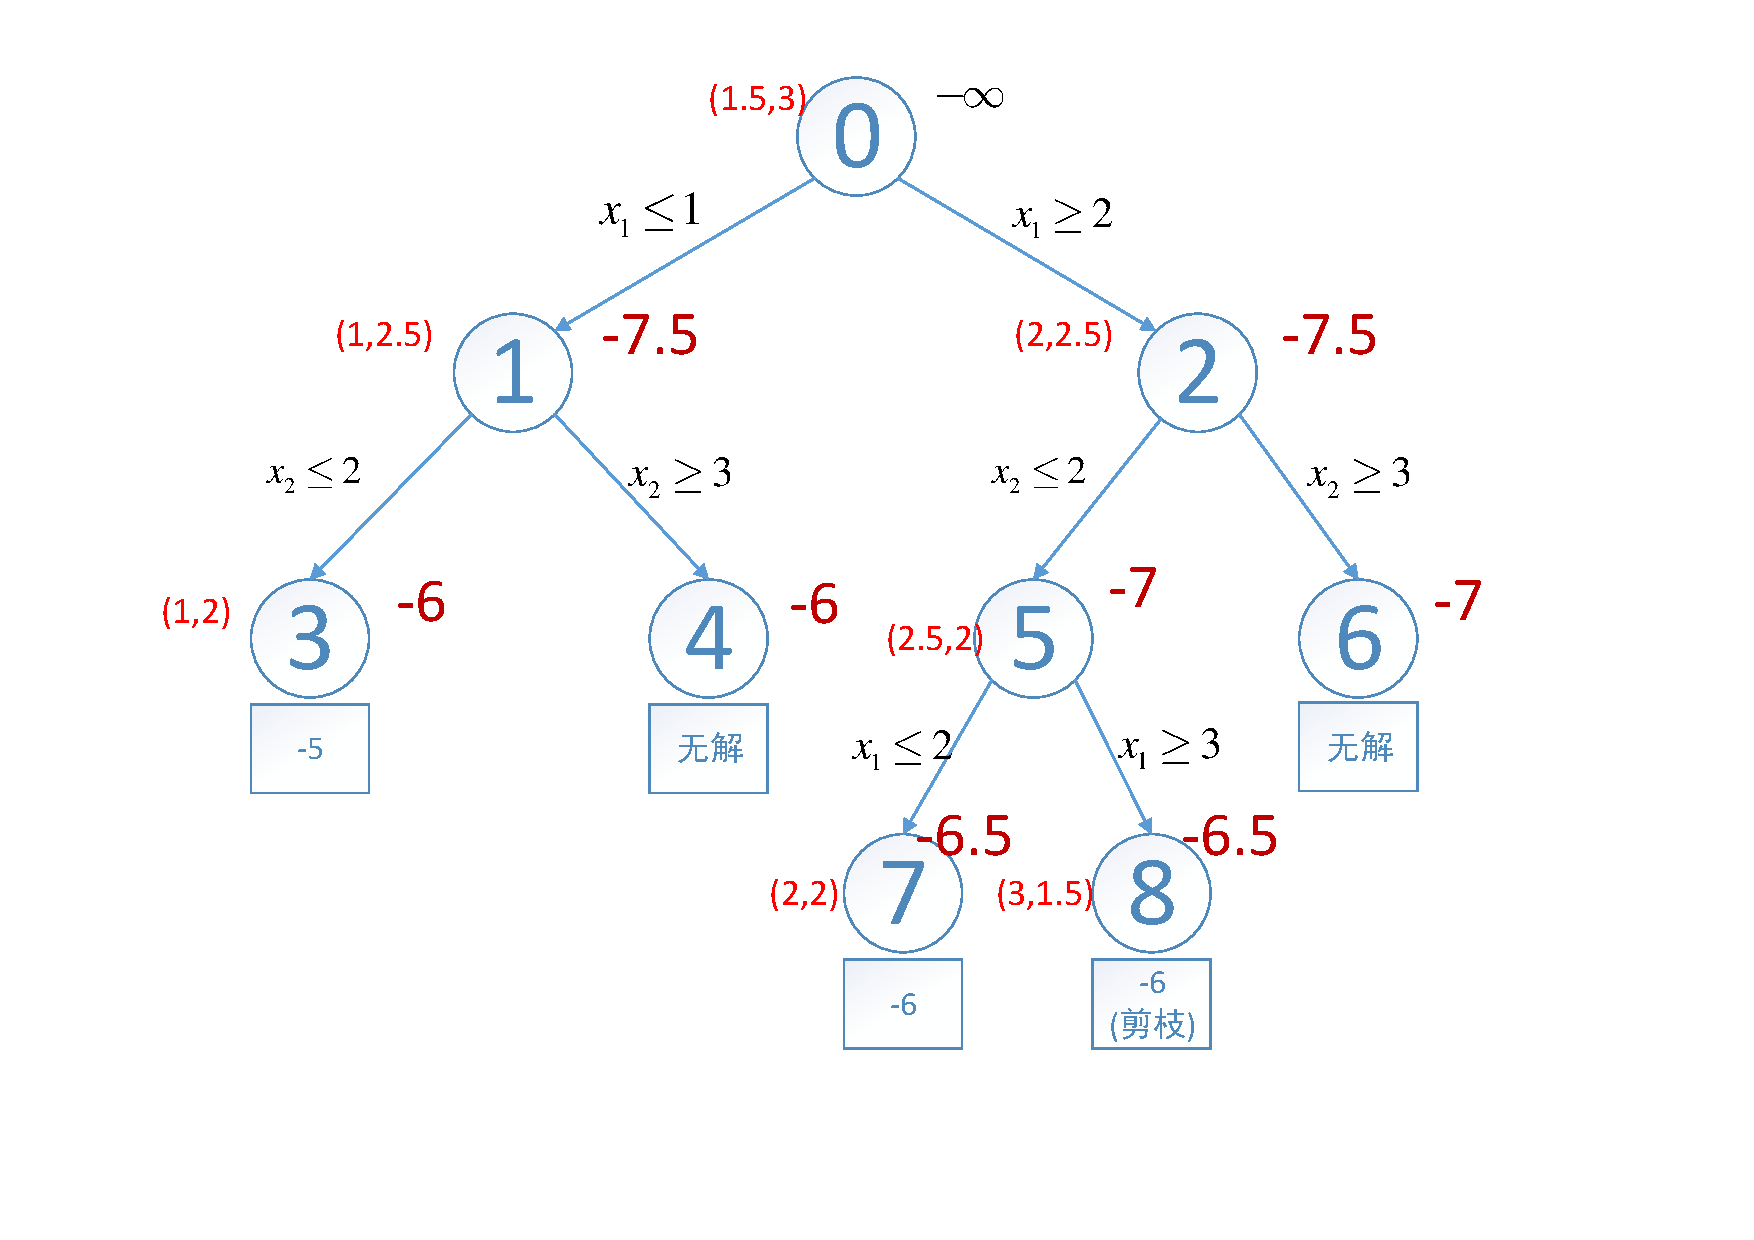
\includegraphics[width=12cm]{4.pdf}
\caption{枚举树}
\end{figure}
\end{enumerate}

\end{document}
